\documentclass[revision-guide.tex]{subfiles}
%% Current Author: PS
\setcounter{chapter}{2}
\begin{document}
\chapter{Deformation of Solids}
\section*{Content}
\begin{itemize}
\item elastic and plastic behaviour
\item stress and strain
\end{itemize}

\section*{Candidates should be able to:}
\spec{distinguish between elastic and plastic deformation of a material}

Elastic deformation is defined as deformation where the sample returns to its original length when the load is removed. Plastic deformation involved a permanent change in length of the sample.

\spec{recall the terms brittle, ductile, hard, malleable, stiff, strong and tough, explain their meaning and give examples of materials exhibiting such behaviour}

\begin{description}
    \item[Brittle] Brittleness is an indicator of how soon after the yield point a material fractures. Failure will be through the propagation of cracks. A brittle material cannot absorb much energy before breaking. For example, glass and ceramics can be strong but brittle.
    \item[Ductile] Ductility is a measure of plastic behaviour under tension. It gives an indication of how easily a material can be drawn into wires i.e. can withstand large strains without breaking. Copper is highly ductile.
    \item[Hard] Hardness is a measure of a materials ability to resist impact or scratching. Diamond is an exceptionally hard material.
    \item[Malleable] Malleability is a measure of plastic behaviour under compression. It gives an indication of how easily a material can be worked. Metals are ductile and hence relatively easy to form into shapes for use in manufacture.
    \item[Stiff] Stiffness measures how much a material resists deformation. A measure of stiffness is the Young Modulus. Glass fibres and steel are both stiff materials.
    \item[Strong] A strong material is able to withstand a large stress without failing.
    \item[Tough] Toughness is a measure of the ability of a material to resist failure through crack propagation. It is the opposite of brittleness. A tough material is able to absorb a lot of energy without breaking. Plastics/polymers are often tough.
\end{description}

\spec{explain the meaning of,  and recall and use the appropriate equations to calculate tensile/compressive stress, tensile/compressive strain, spring constant, strength, breaking stress, stiffness and Young modulus}

Firstly, compressive forces and deformations are those which reduce the length of the sample whereas tensile forces act to increase its length.

\begin{description}
    \item[Stress] Stress is defined as the force per unit of cross-sectional area applied to a material. \[ \sigma = \frac{F}{A} \] Stress is measured in pascals (Pa).
    \item[Strain] Strain is the fractional extension of a material. \[ \epsilon = \frac{x}{l} \]
    where $l$ is the original length.
    \item[Spring constant] The spring constant $k$ is the force per unit of extension of a material during its proportional phase of deformation. It is defined by Hooke's Law: \[ F = kx\] The spring constant is often used as a measure of stiffness of an object.
    \item[Strength] Strength is often measured as the maximum stress a material can withstand before permanent deformation. This is known as the yield stress.
    \item[Breaking stress] This is the stress at which the material fails.
    \item[Young modulus] This is a quantitative measure of the stiffness of a material, defined as stress per unit of strain in the proportional region the material's behaviour. \[ E = \frac{\sigma}{\epsilon} \]
\end{description}

\spec{draw force-extension, force-compression and tensile/compressive stress-strain graphs, and explain the meaning of the limit of proportionality, elastic limit, yield point, breaking force and breaking stress}

The gradient of a force-extension graph gives the spring constant.

\begin{figure}[ht]
    \begin{center}
        \begin{tikzpicture}[scale=1]
            \draw[->] (-0.5,0) -- (10,0) node[anchor=north] {$\epsilon$};
            \draw[->] (0,-0.5) -- (0,6) node[anchor=east] {$\sigma$};
            \draw (0,0) -- (1.5,3) .. controls (2,3.5) .. (2.5,3) .. controls (3,2.8) .. (4,4) .. controls (5.5,5.5) and (8,5.5) .. (10,4.5);
            \fill (1.5,3) circle (2pt) node[anchor=south east] {A};
            \fill (2,3.4) circle (2pt) node[anchor=south] {B};
            \fill (7,5.2) circle (2pt) node[anchor=south] {C};
            \fill (10,4.5) circle (2pt) node[anchor=south] {D};
            \node[draw, text width = 4cm] at (13,3) {
            \begin{description}
                \item[A] The limit of proportionality
                \item[B] The yield point
                \item[C] The ultimate stress (maximium stress)
                \item[D] The breaking point
            \end{description}
            };
        \end{tikzpicture}
    \end{center}
    \caption{Stress-strain curve for a ductile material}
    \label{stress-strain}
\end{figure}

Figure \ref{stress-strain} shows an example stress-strain curve. Note that the limit of proportionality is often a good approximation of the elastic limit of a metal. The ``breaking stress'' usually refers to the ultimate stress, i.e. the maximum stress the material can withstand, rather than the stress at the breaking point.

\spec{state Hooke's law and identify situations in which it is obeyed}

\[ F = kx \]

Hooke's law is obeyed by an ideal spring and by a sample of metal up to the limit of proportionality.

\spec{account for the stress-strain graphs of metals and polymers in terms of the microstructure of the material.}

\subsection{Metals}
Metals consist of positive ions in a sea of delocalised electrons. During the elastic phase of deformation the spaces between the ions get larger and smaller. The metallic bonds resist this change from their equilibrium length and act like small springs acting to return the spacing to its original length.

An initial expectation of the plastic phase of deformation in a metallic lattice may be that the planes of ions slip past one another; however an analysis of the forces required for such movement gives an answer hundreds of times higher than the measured yield stress. Instead, the plastic deformation of metals must be explained in terms of \emph{dislocations}. A dislocation occurs when there is a gap in the metallic lattice. Dislocations occur naturally in materials and enable plastic deformation to occur through the breaking of individual bonds in succession, rather than all at once.

\begin{figure}[h]\begin{center}
    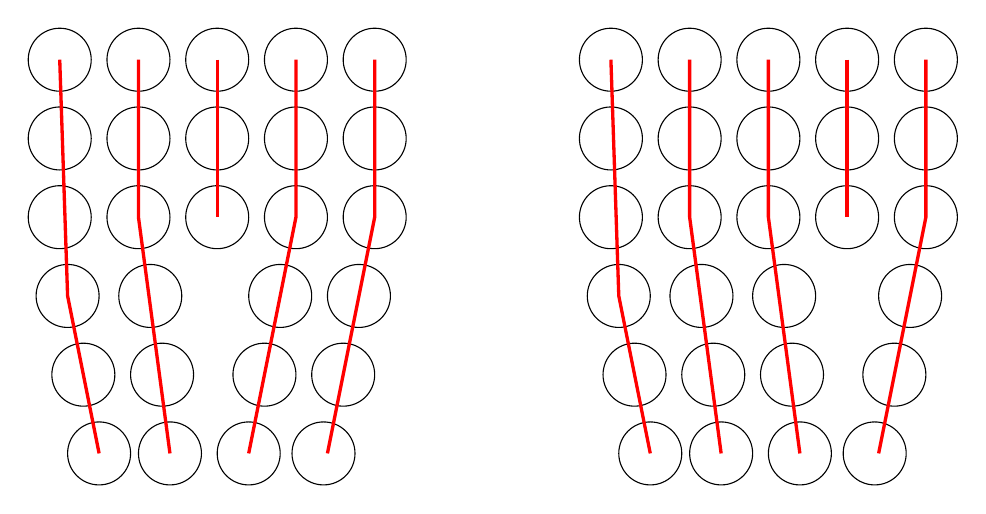
\begin{tikzpicture}
        % Left hand
        \foreach \y in {5,6,7} {
            \foreach \x in {0,1,2,3,4} {
                \draw (\x,\y) circle (4mm);
            }
        }
        \foreach \x in {0.1,1.15,2.8,3.8} {
                \draw (\x,4) circle (4mm);
            }
        \foreach \x in {0.3,1.3,2.6,3.6} {
            \draw (\x,3) circle (4mm);
        }
        \foreach \x in {0.5,1.4,2.4,3.35} {
            \draw (\x,2) circle (4mm);
        }
        \draw[red, very thick] (0,7) -- (0.1,4) -- (0.5,2);
        \draw[red, very thick] (1,7) -- (1,5) -- (1.4,2);
        \draw[red, very thick] (2,7) -- (2,5);
        \draw[red, very thick] (3,7) -- (3,5) -- (2.4,2);
        \draw[red, very thick] (4,7) -- (4,5) -- (3.4,2);
         % right hand
        \foreach \y in {5,6,7} {
            \foreach \x in {7,8,9,10,11} {
                \draw (\x,\y) circle (4mm);
            }
        }
        \foreach \x in {7.1,8.15,9.2,10.8} {
                \draw (\x,4) circle (4mm);
            }
        \foreach \x in {7.3,8.3,9.3,10.6} {
            \draw (\x,3) circle (4mm);
        }
        \foreach \x in {7.5,8.4,9.4,10.35} {
            \draw (\x,2) circle (4mm);
        }
        \draw[red, very thick] (7,7) -- (7.1,4) -- (7.5,2);
        \draw[red, very thick] (8,7) -- (8,5) -- (8.4,2);
        \draw[red, very thick] (9,7) -- (9,5) -- (9.4,2);
        \draw[red, very thick] (10,7) -- (10,5);
        \draw[red, very thick] (11,7) -- (11,5) -- (10.4,2);
    \end{tikzpicture}
    \caption{The movement of a dislocation}\label{disloc}
\end{center}\end{figure}

Figure \ref{disloc} shows a dislocation moving within a metal which would allow the metal to deform by moving one atom at a time. As the movement of dislocations is the dominant mode of plastic deformation, changes to the ability of dislocations to move through the metal have significant effects on it properties. For example:
\begin{description}
    \item[Work Hardening] As a metal is deformed, the dislocations move through the structure. Slowly the dislocations reach grain-boundaries or other dislocations and are no longer able to move. The metal therefore becomes less ductile and more brittle. This may be a desired property in order to harden a metal, or the additional brittleness may be undesirable.
    \item[Alloying] The addition of alloying atoms to the lattice can `pin' a dislocation in place (as shown in figure \ref{alloying}. The metal is therefore no longer able to deform by the movement of dislocations so the metal has a greater yield stress and is less ductile. Examples include adding carbon to iron to produce steel or adding zinc to copper to produce brass.
\end{description}
\begin{figure}[h]\begin{center}
    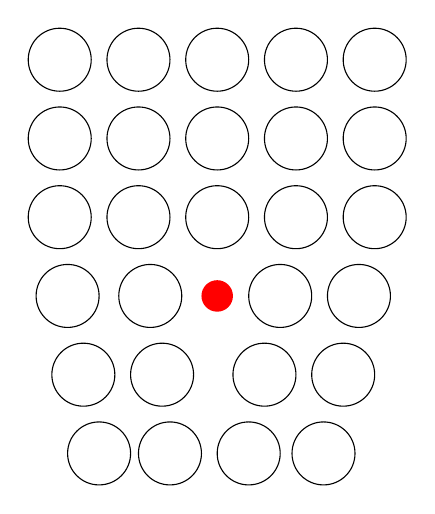
\begin{tikzpicture}
        % Left hand
        \foreach \y in {5,6,7} {
            \foreach \x in {0,1,2,3,4} {
                \draw (\x,\y) circle (4mm);
            }
        }
        \foreach \x in {0.1,1.15,2.8,3.8} {
                \draw (\x,4) circle (4mm);
            }
        \foreach \x in {0.3,1.3,2.6,3.6} {
            \draw (\x,3) circle (4mm);
        }
        \foreach \x in {0.5,1.4,2.4,3.35} {
            \draw (\x,2) circle (4mm);
        }
        \fill [red] (2,4) circle (2mm);
    \end{tikzpicture}
    \caption{Alloying atom pinning a dislocation}\label{alloying}
\end{center}\end{figure}

The effect on a stress-strain graph can be seen in figure \ref{stress-strain-alloy} below.

\begin{figure}[ht]
    \begin{center}
        \begin{tikzpicture}[scale=0.5]
            \draw[->] (-0.5,0) -- (10,0) node[anchor=north] {$\epsilon$};
            \draw[->] (0,-0.5) -- (0,8) node[anchor=east] {$\sigma$};
            \draw (0,0) -- (1.5,3) .. controls (2,3.5) .. (2.5,3) .. controls (3,2.8) .. (4,4) .. controls (5.5,5.5) and (8,5.5) .. (10,4.5) node[anchor=north] {Pure metal};
            \fill (10,4.5) circle (1mm);
            \draw (0,0) -- (1.3,5.5) .. controls (1.5,5.8) .. (2,6) node[anchor=south] {Alloy};
            \fill (2,6) circle (1mm);
        \end{tikzpicture}
    \end{center}
    \caption{Stress-strain curve for a ductile material}
    \label{stress-strain-alloy}
\end{figure}

\subsection{Polymers}

Polymers consist of long chain molecules weakly held together by intermolecular forces. Initially the molecules are likely to be tangled-up together. As force is applied it is initially difficult to move the polymer chains from this state (\textbf{A}). As the chains begin to unravel they straighten out by bond rotation, requiring relatively little force for a large increase in strain (\textbf{B}). As the polymer chains become straight it becomes much more difficult to extend the material any further without damaging the material (\textbf{C}).

\begin{figure}[ht]
    \begin{center}
        \begin{tikzpicture}[scale=.75]
            \draw[thick, ->] (-0.5,0) -- (11,0) node[anchor=north] {$\epsilon$};
            \draw[thick, ->] (0,-0.5) -- (0,9) node[anchor=east] {$\sigma$};
            \draw (0,0) .. controls (3,7) and (6,1) .. (10,8);
            \draw (1.5,1) node{\textbf{A}};
            \draw (5,1) node{\textbf{B}};
            \draw (8.5,1) node{\textbf{C}};
            \draw[dashed] (3,0) -- (3,3.6);
            \draw[dashed] (7.2,0) -- (7.2,4.7);
        \end{tikzpicture}
    \end{center}
    \caption{Stress-strain curve for a polymer}
    \label{stress-strain-polymer}
\end{figure}




\end{document}
